% 20200719
\documentclass[../thesis.tex]{subfiles} %% use packages & commands as this main file
\begin{document}
\section{Result}
Biomass densities were stable within days in destructive systems (Fig.\ref{f:destCarbon}).  
Numerical simulation showed stability in biomass densities on destructive harvest systems for both \PoN\ and \PBN\ (Fig.\ref{f:destCarbon}).  \Phy-only systems had linear accumulation of organic carbon while \pbs\ had a stable pool size after an initial drop (Fig.\ref{f:destCarbon}A).  Average yield was stabilized to a non-significant level after day 5 (Fig.\ref{f:ydDaily}A \& \ref{f:ydByHarv}A; p $>$ 0.1 for \PoN\ day 5 \& 50).  Yield stability was not established in \pbs.

Among the four system sets within the LHS scenarios (1.1 million), feasible (for continuous harvest systems) and favourable (for destructive harvest systems) were counted.  Feasible systems had positive yields under analytical calculation of stable positions.  88.3\% (n=971039) \PoH\ and 0.3\% (n=3251) of \PBH\ systems were feasible.  Favourable systems had yield in stable position more than initial values in numerical integration.  99.5\% (n=1094500) \PoN\ systems and 47.0\% (n=517113) \PBN\ systems were favourable.  Compare the number of feasible/favourable systems with the maximum yield (Fig.\ref{f:bacEffect}), \phy-only systems were easy to construct.  Yet a fit \bac\ candidate could also bring up carbon yield (Fig.\ref{f:harvPB}).

\PBH, \PoH, \PBN\ and \PoN\ were significantly different from each other by pairwise Wilcox test (p $\ll$ 0.01) although \phy-only systems looked similar (Fig.\ref{f:harvPo}).  Hence we used \PoN\ systems to represent all \phy-only systems because \phy-only systems were not biologically different.

Biological parameters for \phy\ (Fig.\ref{f:bacEffect}A-D) had unidirectional influence over \phy-only systems.  No parameters had influence on log yield distributions of \pbs s (Fig.\ref{f:bacEffect} \& \ref{f:harvPB}) because most scenarios had zero yield.   As for \phy\ biological parameters, only intraspecific interference ($\aP$) had a decreasing effect on yield.  Density-insensitive \phy\ had higher productivity than others; maximum yield hence concentrated at the minimum of $\aP$.  The other three \phy\ parameters (i.e. $\ePR$, $\eP$ and $\gP$) had a stable positive influence on log yield fluxes.  \Phy\ biological parameters had no observational effect on \pbs s.  The reason was because unfeasible scenarios dominated the distributions.

Biological parameters for \bac\ (Fig.\ref{f:bacEffect} \& \ref{f:harvPB}) had no observable influence over all systems.  Since these four parameters had no mathematical effect on \phy-only systems (equilibrium 3 in Table \ref{t:eqm}), fluctuations from \phy-only systems in Fig.\ref{f:bacEffect}E-H was due to LHS sampling effect.  Due to the dominance of unfeasible scenarios, no observational effect were on \pbs s.

Log yield distributions for \phy-only systems were stable with large ranges regardless of harvest mode (Fig.\ref{f:ydByHarv}B).  \PBN\ systems were the only system with unfavourable harvest intervals (median -0.00001, IQR [-0.00025 - +0.00106]\dxdt).  \PoH\ and \PoN\ had similar maximum yields of 345\dxdt ($T$ = 19900 for \PoN; $x$ = 19501 for \PoH).  Maximum yield for \PBH\ systems was 285 ($x$ = 2101) \dxdt\ and that for \PBN\ systems was 243 ($T$ = 90) \dxdt.  All maximum yield scenarios were outliers.  Similar sets of \phy\ features led to maximum yields in \phy-only and \pbs s (Fig.\ref{f:bacEffect}A-D).  Maximum yield systems preferred high carbon to biomass conversion efficiency (both $\ePR$ \& $\eP$ high values) under moderate-high growth rate and minimal population density sensitivity.  Although bacteria only appeared in \pbs s, requirements for maximum yield were different between \PBN\ and \PBH\ (Fig.\ref{f:harvPB}E-H).  A \PBN\ system required high leakage \bac\ (high $\eBR$ \& low $\eB$) with very high growth rate and high death rate.  \PBH\ systems needed a balanced carbon to biomass level (moderate $\eBR$ \& moderate $\eB$), high growth and low death rates \bac.  In short, requirement for the best \bac\ was strict and specific according to the harvest mode; \phy\ requirements were comparatively relaxed.

\begin{figure}[H]
    \centering
    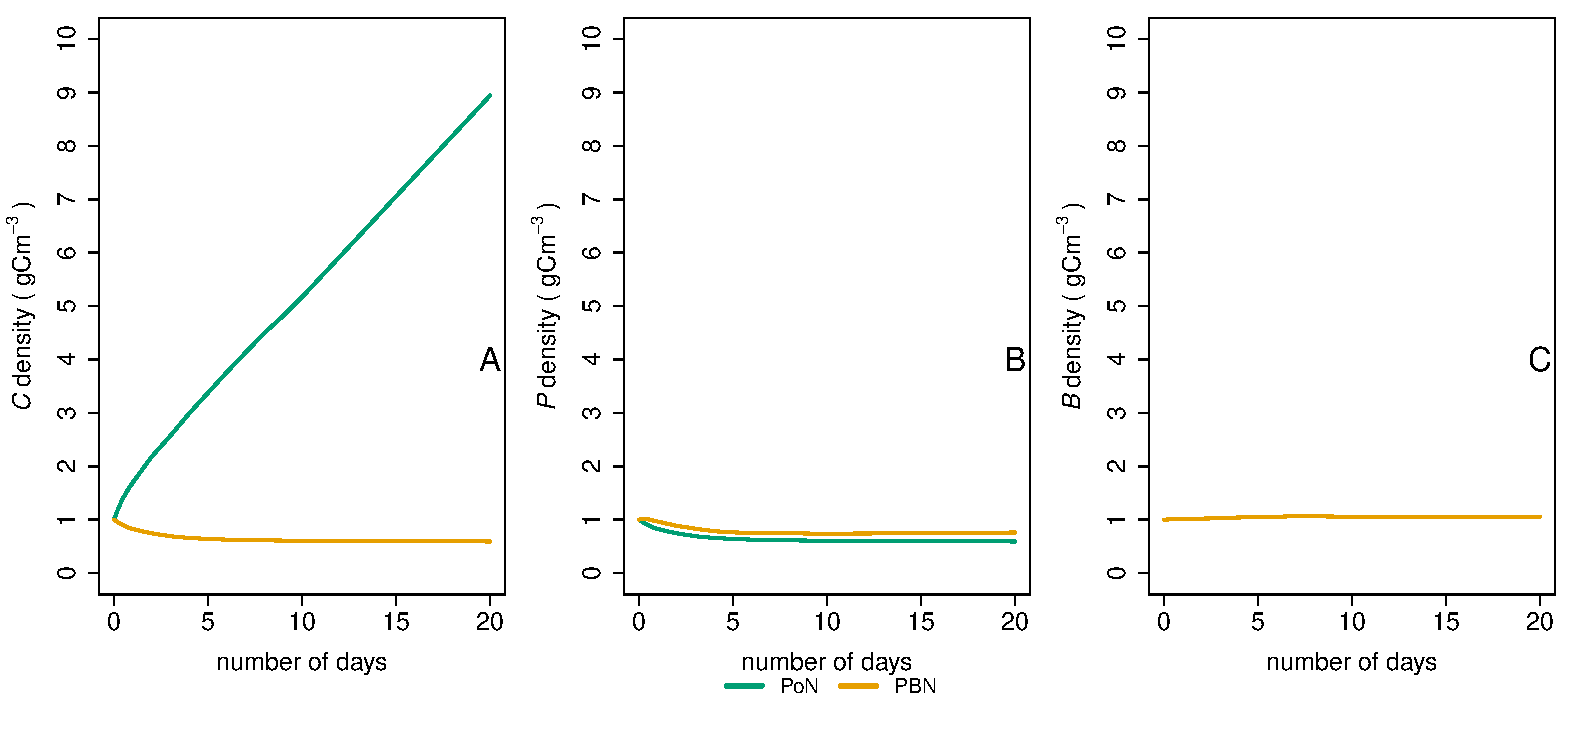
\includegraphics[width=\linewidth]{result/Sample.pdf}
    \caption[Median carbon content in destructive systems]{Median carbon content in destructive systems.  $C$, $P$ and $B$ were carbon pools in Fig.\ref{f:model}.  Eq.\ref{eq:PBH} was used with different initial carbon densities to address the \PoN\ and \PBN\ modes.  Initial carbon densities for \PoN\ were [1,1,0]\den\ ($C$, $P$, $B$) and that for \PBN\ were [1,1,1]\den.  Note that both systems had similar levels of \phy\ across time \textbf{(B)}.  Yet due to the presence of \bac\ \textbf{(C)}, organic carbon pool density changes were huge \textbf{(A)}.  Also note that after a initial boost, accumulation of organic carbon was linear for \PoN\ \textbf{(A)}.  Note that existence of \bac\ suppressed the organic carbon density in the system \textbf{(A)} with almost unchanged \bac\ biomass density \textbf{(C)}.}
    \label{f:destCarbon}
\end{figure}

\begin{figure}[H]
    \centering
    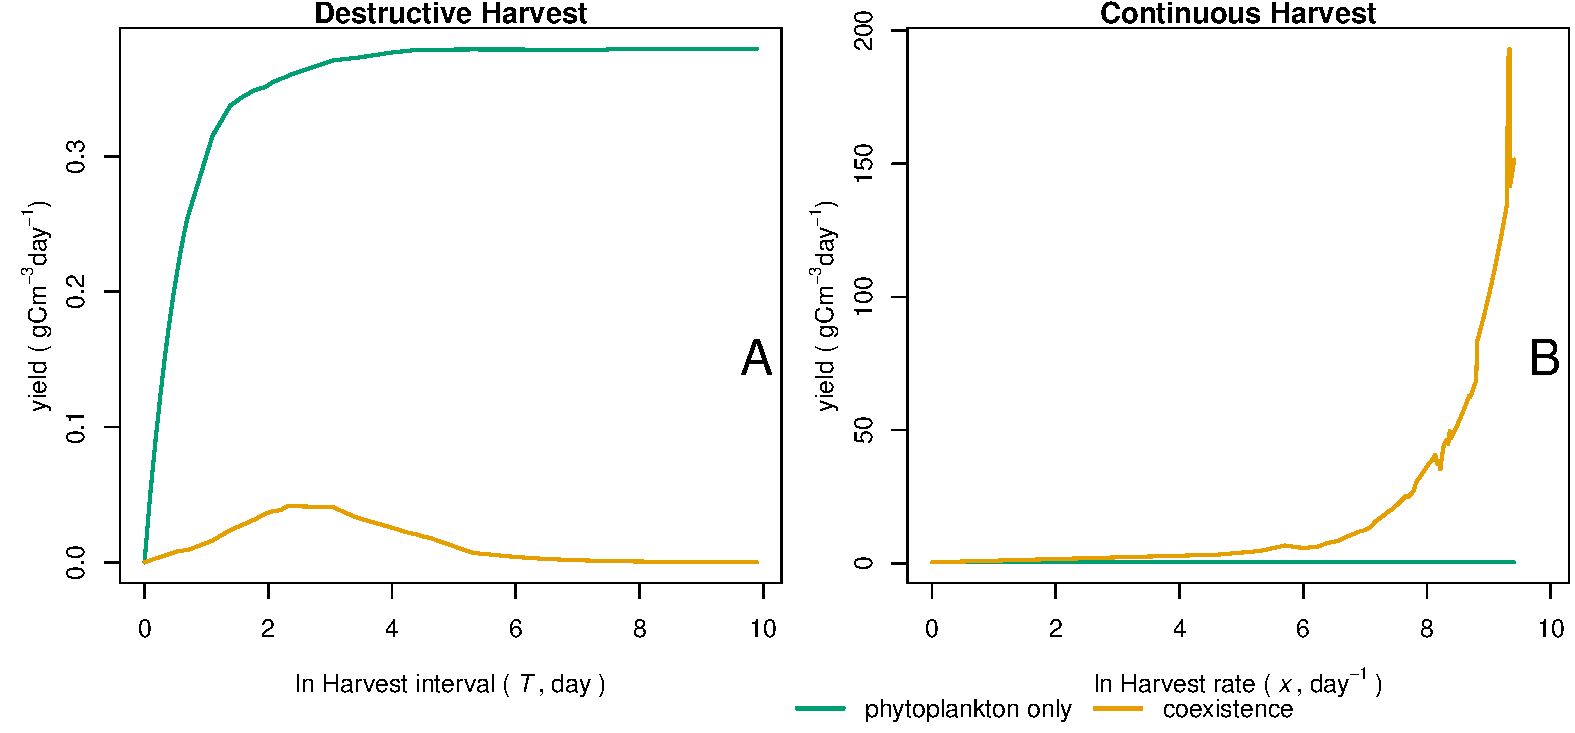
\includegraphics[width=\linewidth]{result/DailyYield.pdf}
    \caption[Median daily yield across systems]{Median daily yield across systems.  Note that both harvest interval/rate were natural logged to emphasize daily yield changes when carbon was harvested more frequent \textbf{(A)} or less amount \textbf{(B)}.  Also note that lower part of \textbf{(B)} was empty because we did not collect such fine-scaled data.  In plot \textbf{A}, the minimal optimum harvest interval for \PoN\ was around 55 days (i.e. exp(4)) while peak yield achieved at day 20 (i.e. exp(3)) for \PBN.  For continuous harvest \textbf{(B)}, very high daily harvest destabilised \PoH\ systems.  Yet for majority of \PBH\ systems, daily yield was zero because such system only feasible for a tiny portion (0.3\%) of the 1.1 million simulated scenarios.}
    \label{f:ydDaily}
\end{figure}

\begin{figure}[H]
    \centering
    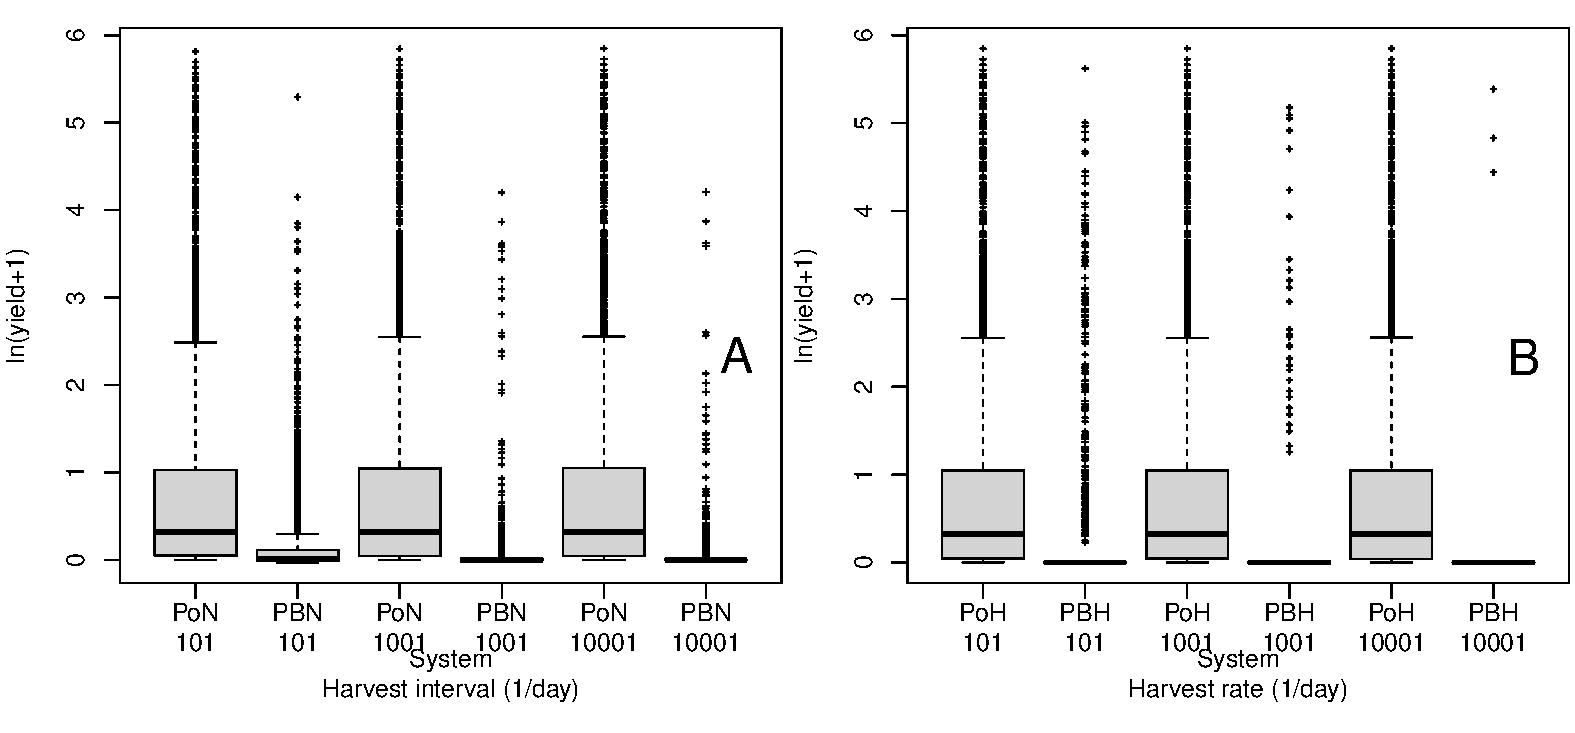
\includegraphics[width=\linewidth]{result/Harvest.pdf}
    \caption[Yield flux distribution by harvest mode]{Log distribution of yield for destructive \textbf{(A)} and continuous \textbf{(B)} harvest modes on selected harvest interval/rates.  \textbf{(A)} Pairwise Wilcox test showed significance (p $\ll$ 0.01) between all except the pair of \PoN\ systems interval 5 and 50 days (p $>$ 0.1).  For \PBN\ systems 0.5 days harvest interval, some systems recorded an initial drop of organic carbon and caused a slight negative yield (none of the drops exhausted the initial organic carbon pool).  The drop recovered in later time with a large variation in yield recovery.  \textbf{(B)} \PoH\ and \PBH\ systems were significantly different (p $\ll$ 0.01).  Significance was also found between \pbs s (p $\ll$ 0.01) but not \phy-only systems (p $>$ 0.1).  Each box represented a sample size of 5500.}
    \label{f:ydByHarv}
\end{figure}

\begin{figure}[H]
    \centering
    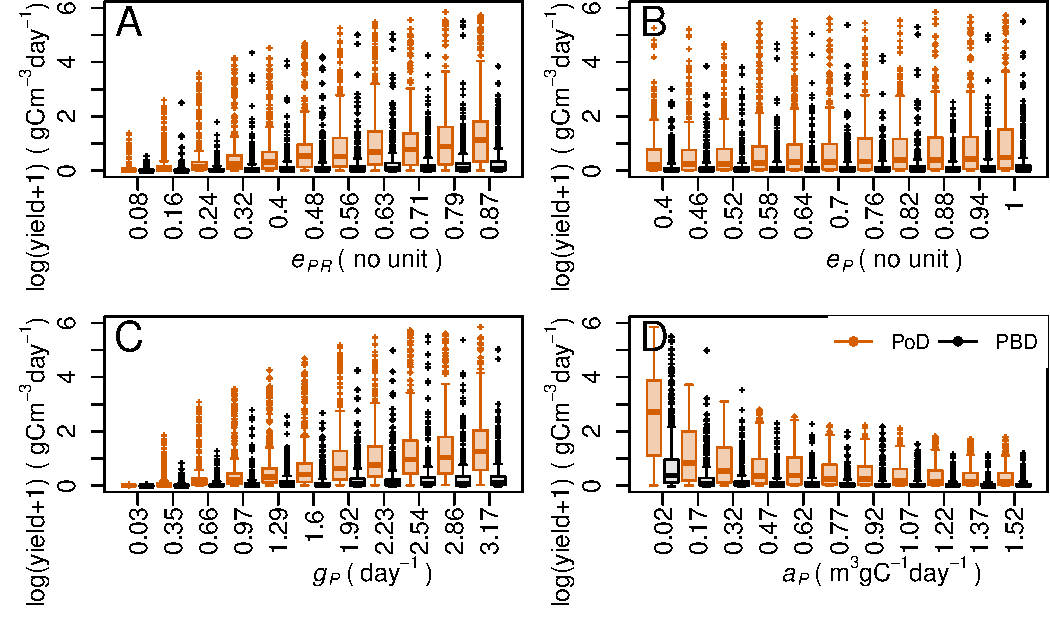
\includegraphics[width=\linewidth]{result/bacEff1.pdf}
    \caption[Log yield flux comparisons between \phy-only and \pbs s on \phy\ parameters]{Log yield flux comparisons between \phy-only and \pbs s on \phy\ parameters along respective parameter ranges under a standardised temperature range of \temp.  Full description of variables were in Table \ref{t:ranges}.  Each group in each plot had an LHS sample size of 5500.  Pairwise Wilcox test showed significance (p $\ll$ 0.01) between the systems.  Note that only a few scenarios of \pbs s were positives, which symbolised small feasibility.  Also note that ranges of both groups were similar, symbolising comparable yield values were possible for \pbs s when biologically compatible candidates were selected.}
    \label{f:bacEffect}
\end{figure}

%\begin{figure}[H]
%    \centering
%    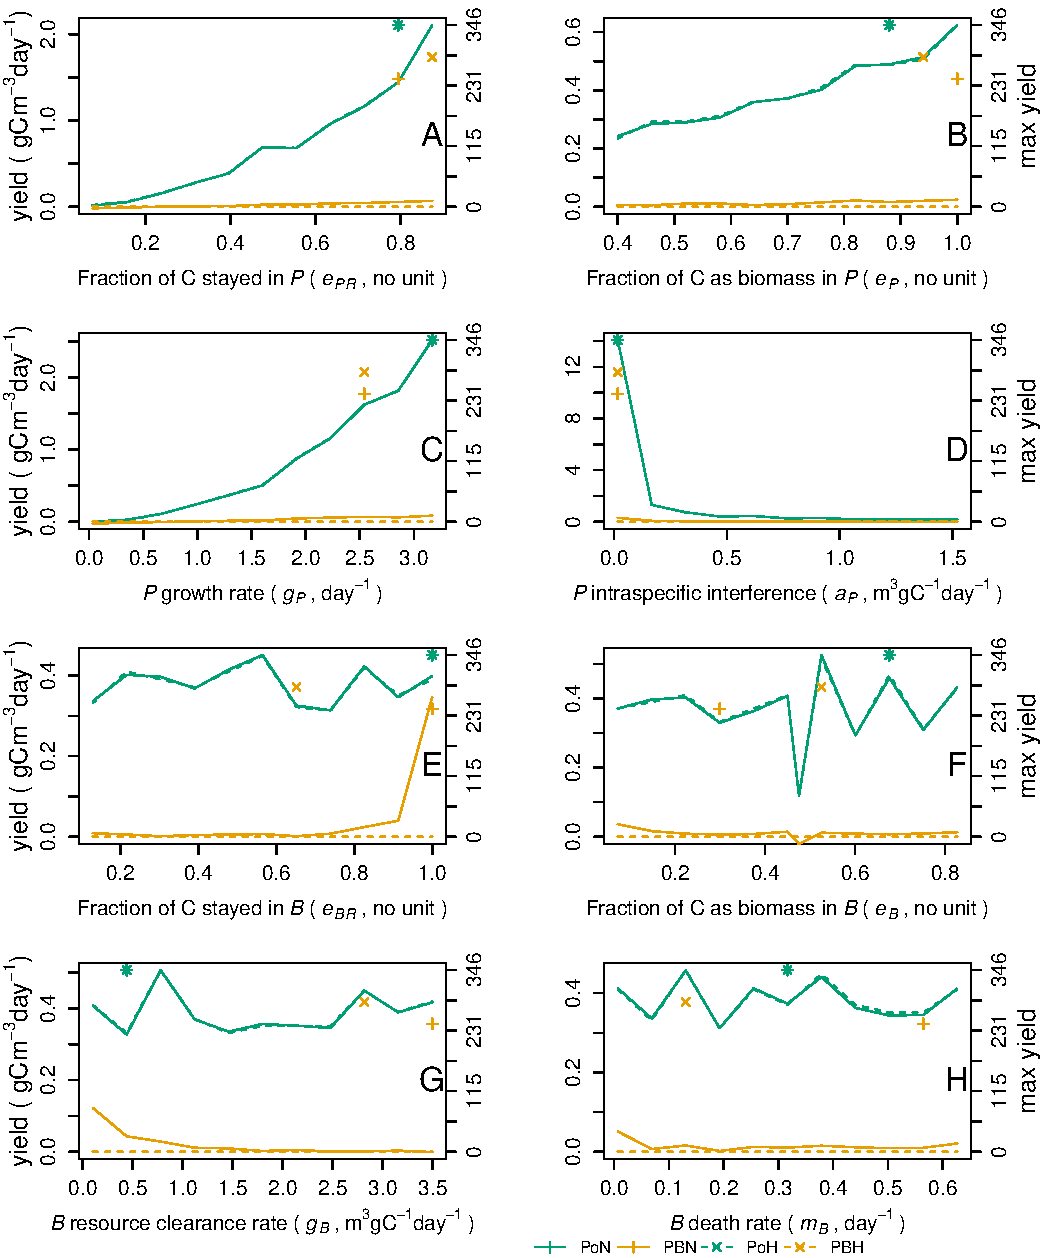
\includegraphics[width=\linewidth]{result/yieldFlux.pdf}
%    \caption[Yield flux median in biological parameter space]{Median yield flux (primary axis) and the maximum yield scenario (secondary axis) along respective parameter ranges under a standardised temperature range of \temp.  Full description of variables were in Table \ref{t:ranges}.  Each median trend had an LHS sample size of 5500.  Pairwise Wilcox test showed significance (p $\ll$ 0.01) between all systems.  Note that trends between \phy-only and \pbs s had different responses while harvest modes only caused small deviation in median yields.  Also note that in all plots, y-axis range for primary axis was much smaller than the secondary axis.  There were many outliers regardless of the parameter under consideration (Fig.\ref{f:ydByHarv}).}
%    \label{f:ydByPara}
%\end{figure}

\end{document}